\section{TF--IDF và hai bộ phân loại tuyến tính}
\label{sec:linear_models}
SVM và Logistic Regression dùng cùng cách tạo đặc trưng từ corpus chuẩn hóa. Sau khi chốt corpus và phép chia, tiêu đề đã phân đoạn được lặp thêm hai lần trước chuỗi tiêu đề--nội dung, tạo ba lần xuất hiện của tiêu đề. Hai notebook dùng danh sách stopword riêng nhưng có cùng nội dung, gồm 1.959 mục sau chuẩn hóa; hash bắt đầu \texttt{8560838c}. Stopword được loại ở bước biểu diễn cho mô hình, không dùng để xác định nhóm trùng của corpus chung.

\subsection{Từ tần suất đến vector thưa}
Với thuật ngữ $j$ và tài liệu $d$, biểu diễn dùng TF logarit, IDF có làm trơn và chuẩn hóa $L_2$:
\begin{align}
\operatorname{tf}_{d,j}&=1+\log n_{d,j}\quad(n_{d,j}>0),\\
\operatorname{idf}_j&=\log\frac{1+N_{train}}{1+\operatorname{df}_j}+1,\\
v_d&=\frac{\operatorname{tf}_d\odot\operatorname{idf}}{\|\operatorname{tf}_d\odot\operatorname{idf}\|_2}.
\end{align}
Từ vựng và IDF chỉ fit trên 139.975 mẫu train. Validation và test đi qua transform với các tham số đã cố định. Cấu hình được chọn giữ unigram và bigram, tối đa 150.000 đặc trưng, \texttt{min\_df=3}, \texttt{max\_df=0.98}; số chiều thực tế là 150.000. Không có SVD trong pipeline này. Các vector được lưu và tính toán dưới dạng thưa, không tạo ma trận dense toàn corpus.

Việc lặp tiêu đề tăng tần suất tín hiệu đầu bài, nhưng hệ số ba không có nghĩa giá trị TF--IDF cuối tăng đúng ba lần: TF logarit và chuẩn hóa $L_2$ còn biến đổi tỷ lệ. Bigram được tạo trên chuỗi ghép, nên cũng có thể xuất hiện ở ranh giới các lần lặp tiêu đề. Toàn văn không bị cắt theo số vị trí như mô hình neural, song thứ tự xa và cấu trúc lập luận không được giữ trong một vector TF--IDF \citep{kowsari2019}.

\subsection{SVM tuyến tính và Logistic Regression}
\texttt{LinearSVC} dùng regularization $L_2$, squared hinge loss và cơ chế một-chống-phần-còn-lại cho 20 lớp. Trong bộ phân loại lớp $c$, nhãn nhị phân $y_{i,c}\in\{-1,+1\}$ tạo hạng mất mát
\begin{equation}
\ell_{i,c}=\bigl[\max(0,1-y_{i,c}(w_c^\top v_i+b_c))\bigr]^2.
\end{equation}
Hệ số $C$ điều khiển đánh đổi regularization và mất mát. Điểm $s_c=w_c^\top v+b_c$ là margin, chưa phải xác suất; nhãn được chọn bằng argmax của 20 điểm. SVM trong thực nghiệm là tuyến tính, khác kernel RBF của một số nghiên cứu ở chương~\ref{chap:related}.

Logistic Regression dùng solver L-BFGS cho phân loại multinomial với regularization $L_2$. Logits tuyến tính được chuẩn hóa thành xác suất lớp:
\begin{equation}
p_c(v)=\frac{\exp(w_c^\top v+b_c)}{\sum_{j=1}^{20}\exp(w_j^\top v+b_j)}.
\end{equation}
Mục tiêu là log-loss có trọng số lớp, khác squared hinge của SVM. Cả hai có cùng thông tin từ vựng, nhưng nghiệm tối ưu và thang điểm khác nhau. Xác suất do LR học vẫn cần kiểm tra calibration; tối ưu log-loss không bảo đảm confidence đúng trên mọi nhóm bài.

\begin{table}[htbp]\centering\small\caption{Hai cấu hình tuyến tính được chọn bằng validation.}\label{tab:linear_config}
\begin{tabular}{lcc}\toprule Thuộc tính & SVM & Logistic Regression\\\midrule
Đặc trưng & \multicolumn{2}{c}{TF--IDF unigram/bigram, 150.000 chiều}\\
Trọng số lớp & balanced & balanced\\
$C$ & 0,5 & 3,0\\
Solver & liblinear, dual auto & L-BFGS\\
Ngưỡng hội tụ & $10^{-4}$ & $10^{-4}$\\
Số vòng tối ưu & 119 & 138\\
Giới hạn vòng & 5.000 & 500\\
Luồng CPU & 4 & 4\\\bottomrule
\end{tabular}\end{table}

\subsection{Đặc trưng học được và giới hạn diễn giải}
Hệ số dương lớn cho biết đặc trưng tăng điểm của lớp trong mô hình đã fit. Với Nông thôn mới, SVM có hệ số 3,1823 cho \texttt{nông\_thôn}; LR có hệ số 13,5690 cho cùng đặc trưng và 6,1810 cho bigram \texttt{xây\_dựng nông\_thôn}. Không so độ lớn giữa hai model như một thang quan trọng chung: mục tiêu, $C$ và thang score khác nhau. Hệ số cũng không phải tác động nhân quả hoặc một lời giải thích đầy đủ cho từng bài.

\begin{figure}[tbp]\centering
\begin{subfigure}[t]{.85\textwidth}\centering
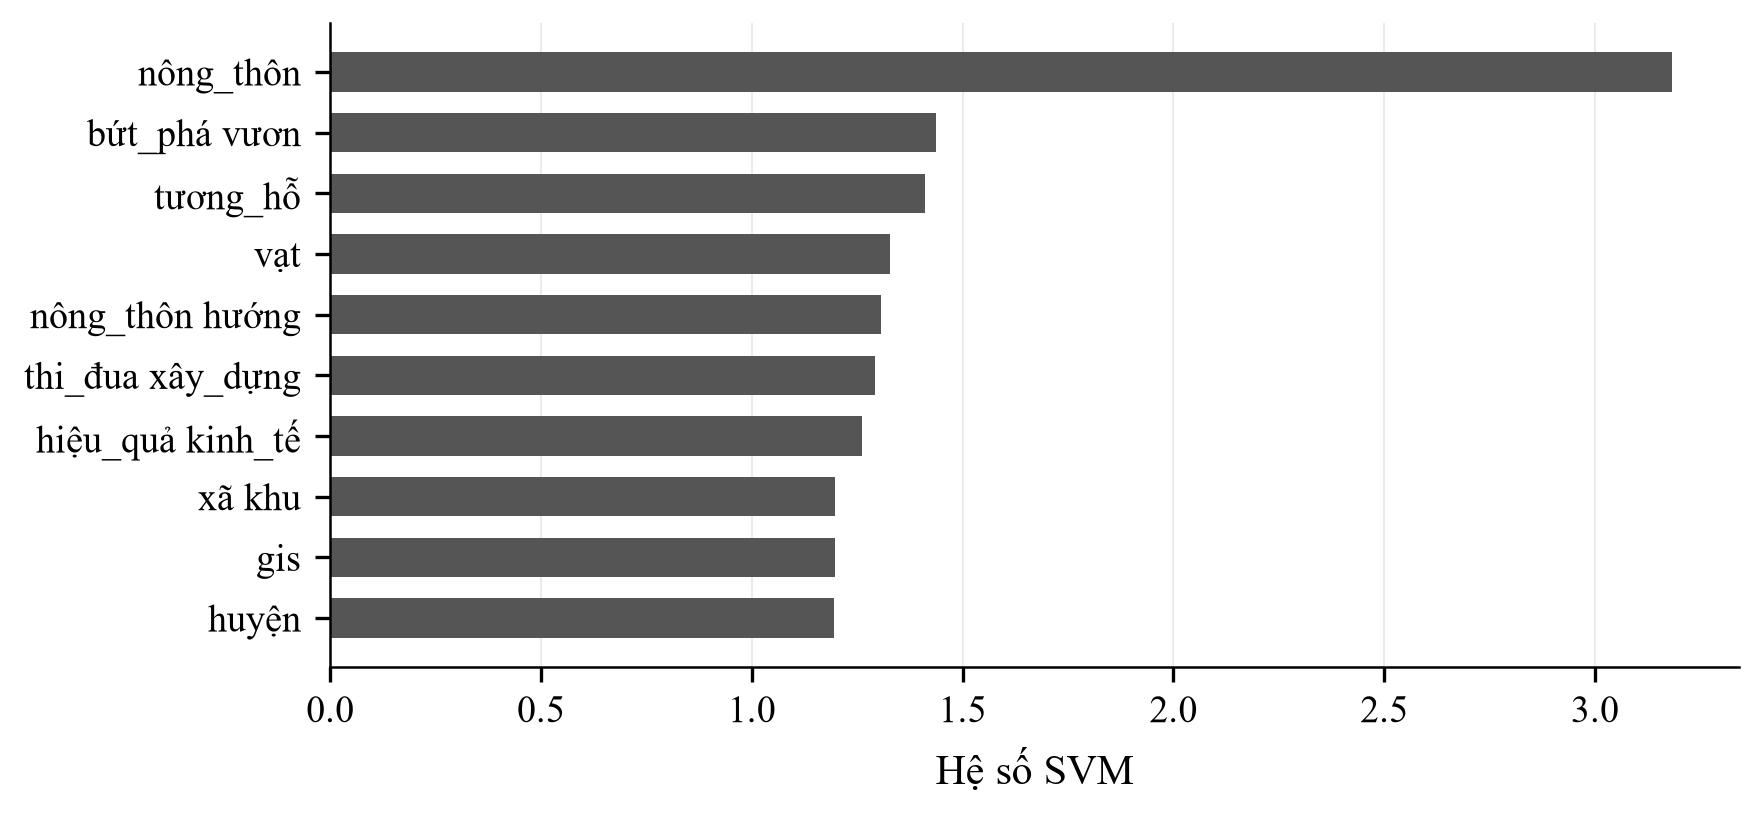
\includegraphics[width=\linewidth]{assets/compact/svm_features.png}\caption{Linear SVM.}\end{subfigure}\par\medskip
\begin{subfigure}[t]{.85\textwidth}\centering
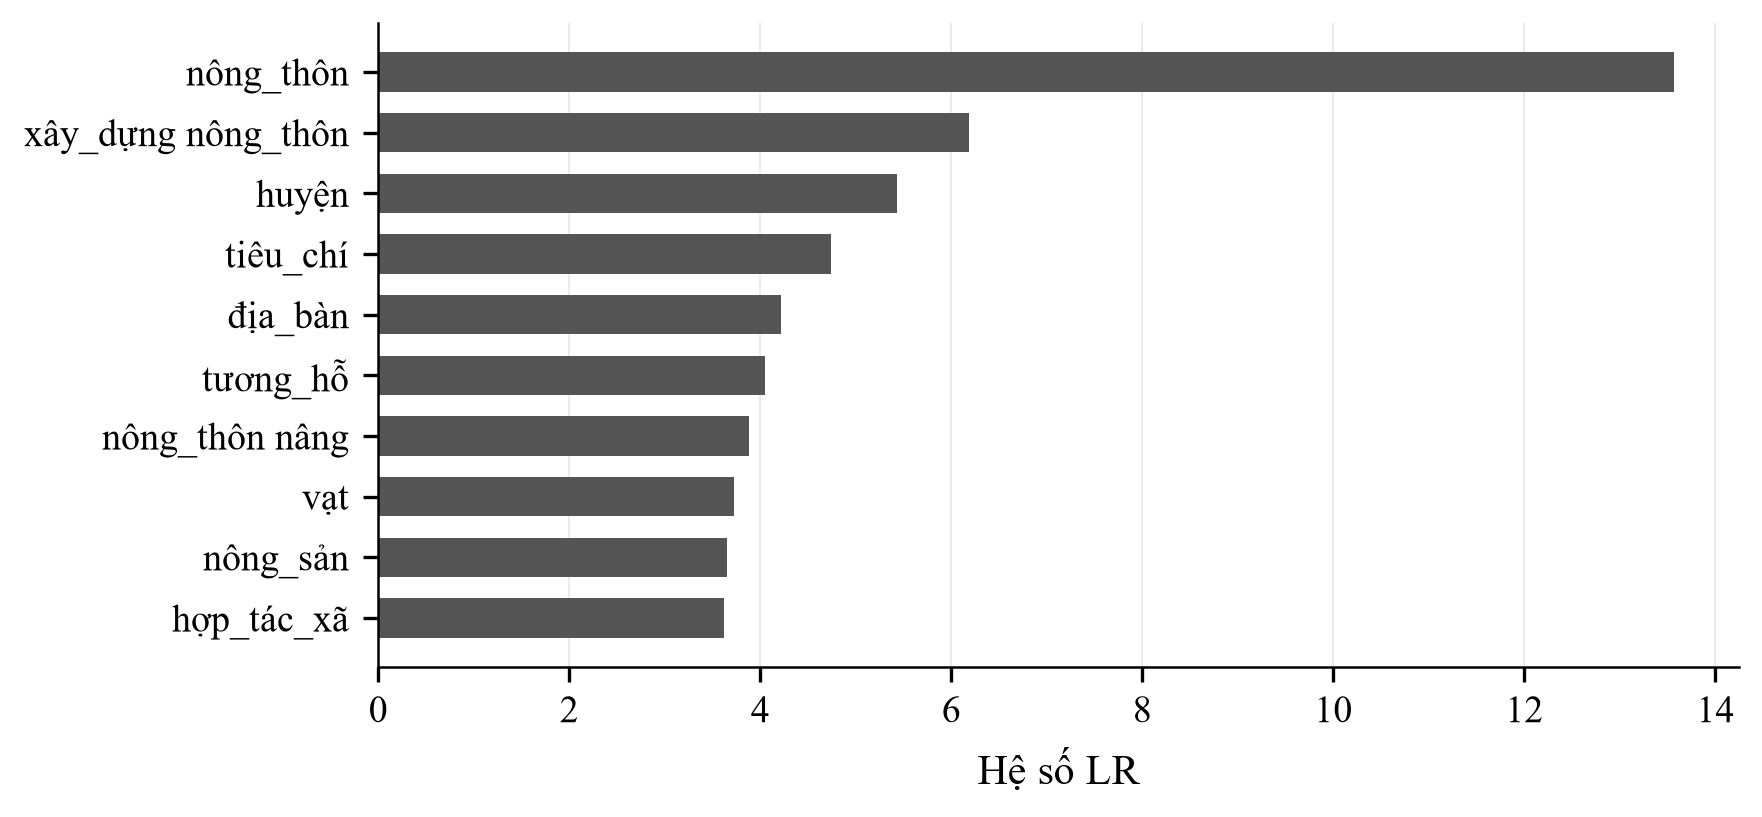
\includegraphics[width=\linewidth]{assets/compact/lr_features.png}\caption{Logistic Regression.}\end{subfigure}
\caption{Đặc trưng có hệ số dương lớn ở Nông thôn mới; thang hệ số không trực tiếp tương đương giữa hai model.}\label{fig:linear-features}\end{figure}

Việc bỏ stopword giảm một phần vốn từ thường xuất hiện, nhưng cũng có thể bỏ tín hiệu diễn ngôn hoặc cách viết của tòa soạn. N-gram còn khai thác cụm cục bộ sau bước lọc, với từ nhiều âm tiết đã được nối bằng PyVi. Vì thế, một bigram là hai đơn vị phân đoạn, không nhất thiết hai âm tiết cách trắng ban đầu. Vocabulary train cố định cũng có thể bỏ thuật ngữ mới ở test; khác biệt này không đồng nhất với UNK của model chuỗi.

Một hệ số lớn không có nghĩa mọi bài chứa term đó phải nhận nhãn tương ứng. Điểm tuyến tính còn cộng các đặc trưng khác và bias, trong khi giá trị term đã qua IDF cùng chuẩn hóa vector. Bỏ một term khỏi một bài có thể thay chuẩn hóa và làm đổi cả vector. Phân tích hệ số cung cấp tín hiệu toàn cục của model được fit, chưa là phép giải thích cục bộ có kiểm soát cho một dự đoán cụ thể.
\FloatBarrier

\section{Biểu diễn chuỗi và kiến trúc BiLSTM}
\label{sec:bilstm}
Phương pháp LSTM trong thiết kế được thực thi bằng biến thể hai chiều BiLSTM. Embedding được khởi tạo và học từ train, không nạp Word2Vec, PhoW2Vec hay encoder tiền huấn luyện. Chuỗi đầu vào giữ stopword và chỉ ghép tiêu đề một lần với nội dung. Vì vậy, đây là một đối chứng học biểu diễn tuần tự có giám sát, khác cả TF--IDF và PhoBERT có pretraining.

\subsection{Vocabulary, từ ngoài từ vựng và Head--Tail}
Vocabulary đếm từ trên train, lấy từ có tần suất ít nhất hai, sắp theo tần suất giảm rồi theo từ điển khi bằng nhau. Tổng 50.000 ID gồm PAD bằng 0, UNK bằng 1 và 49.998 từ. Token ngoài vocabulary được đưa về UNK; embedding PAD không được cập nhật như từ nội dung. Không học vocabulary từ validation/test để giảm tỷ lệ từ lạ một cách không hợp lệ.

Cấu hình được chọn giới hạn 512 \emph{từ đã phân đoạn}. Bài dài giữ 256 từ đầu và 256 từ cuối, không thêm BOS/EOS. Bài ngắn được giữ đầy đủ; mỗi batch pad đến độ dài lớn nhất của các mẫu trong batch, rồi dùng packed sequence để bỏ padding khỏi quá trình recurrent. Head--Tail vẫn bỏ phần giữa và nối hai đoạn không kề nhau, nhưng đơn vị cắt khác 254 subword nội dung của PhoBERT.

Trên corpus 199.965 bài, 44,14\% vượt 512 từ; tỷ lệ từ giữ trung bình là 87,13\%. Hai giá trị được tính từ độ dài đã xuất, không phải một lần tokenize mới. Tỷ lệ OOV trên toàn chuỗi train/validation/test lần lượt là 0,7782\%, 0,8714\% và 0,8696\%. Audit OOV tính trước cắt Head--Tail; không đồng nhất với tỷ lệ UNK trong tensor cuối hoặc lượng thông tin ngữ nghĩa bị mất.


Việc đặt UNK chỉ xử lý khả năng tra ID, không bổ sung nghĩa riêng cho mỗi từ lạ. Những từ ngoài vocabulary khác nhau cùng đi vào một embedding UNK; chúng vẫn có thể được phân biệt một phần bởi các từ bao quanh, nhưng thông tin từ vựng gốc đã mất. Tỷ lệ OOV thấp trên snapshot chưa dự báo tỷ lệ ở tin tương lai chứa tên riêng và thuật ngữ mới.

Packed sequence giúp trạng thái kết thúc phản ánh độ dài thật của bài, tránh recurrent tiếp tục quét nhiều PAD tới độ dài batch. Hai hướng đều quét chuỗi sau Head--Tail; hướng ngược không khôi phục phần giữa đã bị bỏ. Khi nối hai đoạn xa nhau, mô hình vẫn coi chúng là một chuỗi kề nhau, một giả định chung của cách cắt này với PhoBERT.



\subsection{Cơ chế cổng và trạng thái chuỗi}
LSTM duy trì hidden state $h_t$ cùng cell state $c_t$. Forget gate quyết định phần trạng thái cũ giữ lại, input gate điều chỉnh phần thông tin mới ghi vào, output gate điều chỉnh thông tin đưa ra hidden. Dạng cập nhật chuẩn giải thích vai trò của các cổng trong recurrent layer được dùng:
\begin{equation}c_t=f_t\odot c_{t-1}+i_t\odot\widetilde c_t,\qquad h_t=o_t\odot\tanh(c_t).\end{equation}
Các vector gate có giá trị sigmoid và được học từ embedding hiện tại cùng hidden trước đó; candidate cell dùng biến đổi phi tuyến. Đây là trạng thái theo chuỗi, không phải một đặc trưng TF--IDF được coi tùy ý như trục thời gian. Cổng cho phép điều chỉnh truyền thông tin nhưng không bảo đảm nhớ đủ mọi chi tiết qua một bài dài \citep{kowsari2019}.

Hai hướng của BiLSTM có tham số riêng và quét theo hai thứ tự ngược nhau. Chúng cung cấp hai cách tổng hợp cùng chuỗi đã giữ, rồi head nhận vector nối; số lớp recurrent vẫn là một, không biến thành mạng nhiều tầng vì có hai hướng. Dropout bên ngoài recurrent có vai trò regularization, không bổ sung token hoặc tri thức ngôn ngữ tiền huấn luyện.


\subsection{Trạng thái hai chiều và đầu phân loại}
Embedding có chiều 200; một recurrent layer có hidden size 128 cho mỗi hướng. Các cổng forget, input và output lần lượt điều chỉnh thông tin cũ giữ lại, thông tin mới ghi vào cell state và phần trạng thái được xuất theo chuỗi \citep{kowsari2019}. Mô hình quét chuỗi đã cắt ở cả hai hướng, rồi ghép trạng thái kết thúc phép quét xuôi và ngược:
\begin{equation}
r=[\overrightarrow h_{\mathrm{end}};\overleftarrow h_{\mathrm{end}}]\in\mathbb R^{256},\qquad
z=W\operatorname{Dropout}(r)+b\in\mathbb R^{20}.
\end{equation}
Trạng thái kết thúc hướng ngược không phải hidden tại vị trí cuối theo thứ tự đọc xuôi. Code lấy hai hidden cuối của hai hướng từ packed sequence, không lấy trung bình các token. Dropout 0,35 đặt sau embedding và trước lớp tuyến tính; recurrent dropout giữa các layer bằng 0 vì chỉ có một layer.

\begin{figure}[tbp]\centering
\begin{tikzpicture}[box/.append style={text width=23mm,minimum height=15mm}]
\node[box] (ids) at (0,0) {ID từ\\$B\times L$\\$L\le512$};
\node[box] (emb) at (3,0) {Embedding\\$B\times L\times200$};
\node[box] (fw) at (6,1.1) {LSTM xuôi\\$h_{end}\in\mathbb R^{128}$};
\node[box] (bw) at (6,-1.1) {LSTM ngược\\$h_{end}\in\mathbb R^{128}$};
\node[box] (cat) at (9,0) {Ghép hai\\trạng thái\\$B\times256$};
\node[box] (head) at (12,0) {Dropout\\Linear $256\to20$\\Logits};
\draw[flow] (ids)--(emb);
\draw[flow] (emb.east)--++(0.4,0)|-(fw.west);
\draw[flow] (emb.east)--++(0.4,0)|-(bw.west);
\draw[flow] (fw.east)--++(0.3,0)|-(cat.west);
\draw[flow] (bw.east)--++(0.3,0)|-(cat.west);
\draw[flow] (cat)--(head);
\end{tikzpicture}
\caption{BiLSTM thực thi trong notebook: embedding học từ đầu, packed sequence, ghép hidden cuối hai hướng và đầu phân loại 20 lớp. Dropout embedding được lược trong khối để giữ sơ đồ gọn.}
\label{fig:bilstm_arch}
\end{figure}

Model có 10.343.060 tham số: embedding chiếm 10.000.000, BiLSTM 337.920 và classifier 5.140. Phần lớn tham số thuộc bảng từ, không phải recurrent layer. Kích thước nhỏ hơn PhoBERT không tự xác định chất lượng; vocabulary, số từ giữ, cách tổng hợp chuỗi và chế độ pretraining đều khác nhau. Phần tiếp theo trình bày encoder ngữ cảnh và cấu hình PhoBERT được dùng trong cùng bài toán.
